\documentclass{Gesue_PresentationTemplate}

\title{Introduction to literate programming}
\subtitle{a brief introduction}
\date{April 2023}
\author{Riccardo Maria Gesuè}
\institute{Fellowship Of Clean Code}

% insert your instituition logo here
\newcommand{\mylogo}{Images/gssi_logo.jpeg}

\begin{document}
\maketitle
%%%%%%%%%%%
\section{What is literate programming}
\begin{frame}
  \frametitle{What is literate programming}
  \begin{block}{}
    Literate programming is a
    \alert{programming paradigm}
    in which a computer program is given
    as an explanation of how it works in
    \alert{natural language}.
  \end{block}
  \begin{itemize}
    \item \alert{Embedded} snippets of code.
    \item Traditional source code can be
          \alert{generated and compiled}.
    \item Depending on the implementation,
          snippets can be \alert{executed} and their
          output saved and/or printed.
  \end{itemize}
  Literate programming was first introduced in
  1984 by Donald Knuth\cite{knuthliterate}.
  The implementation
  he developed was called WEB\cite{WEB}.
\end{frame}
\begin{frame}
  \frametitle{A first example}
  \begin{block}{}
    Literate programming is the combination of
    documentation and source code.
  \end{block}
  \centering
  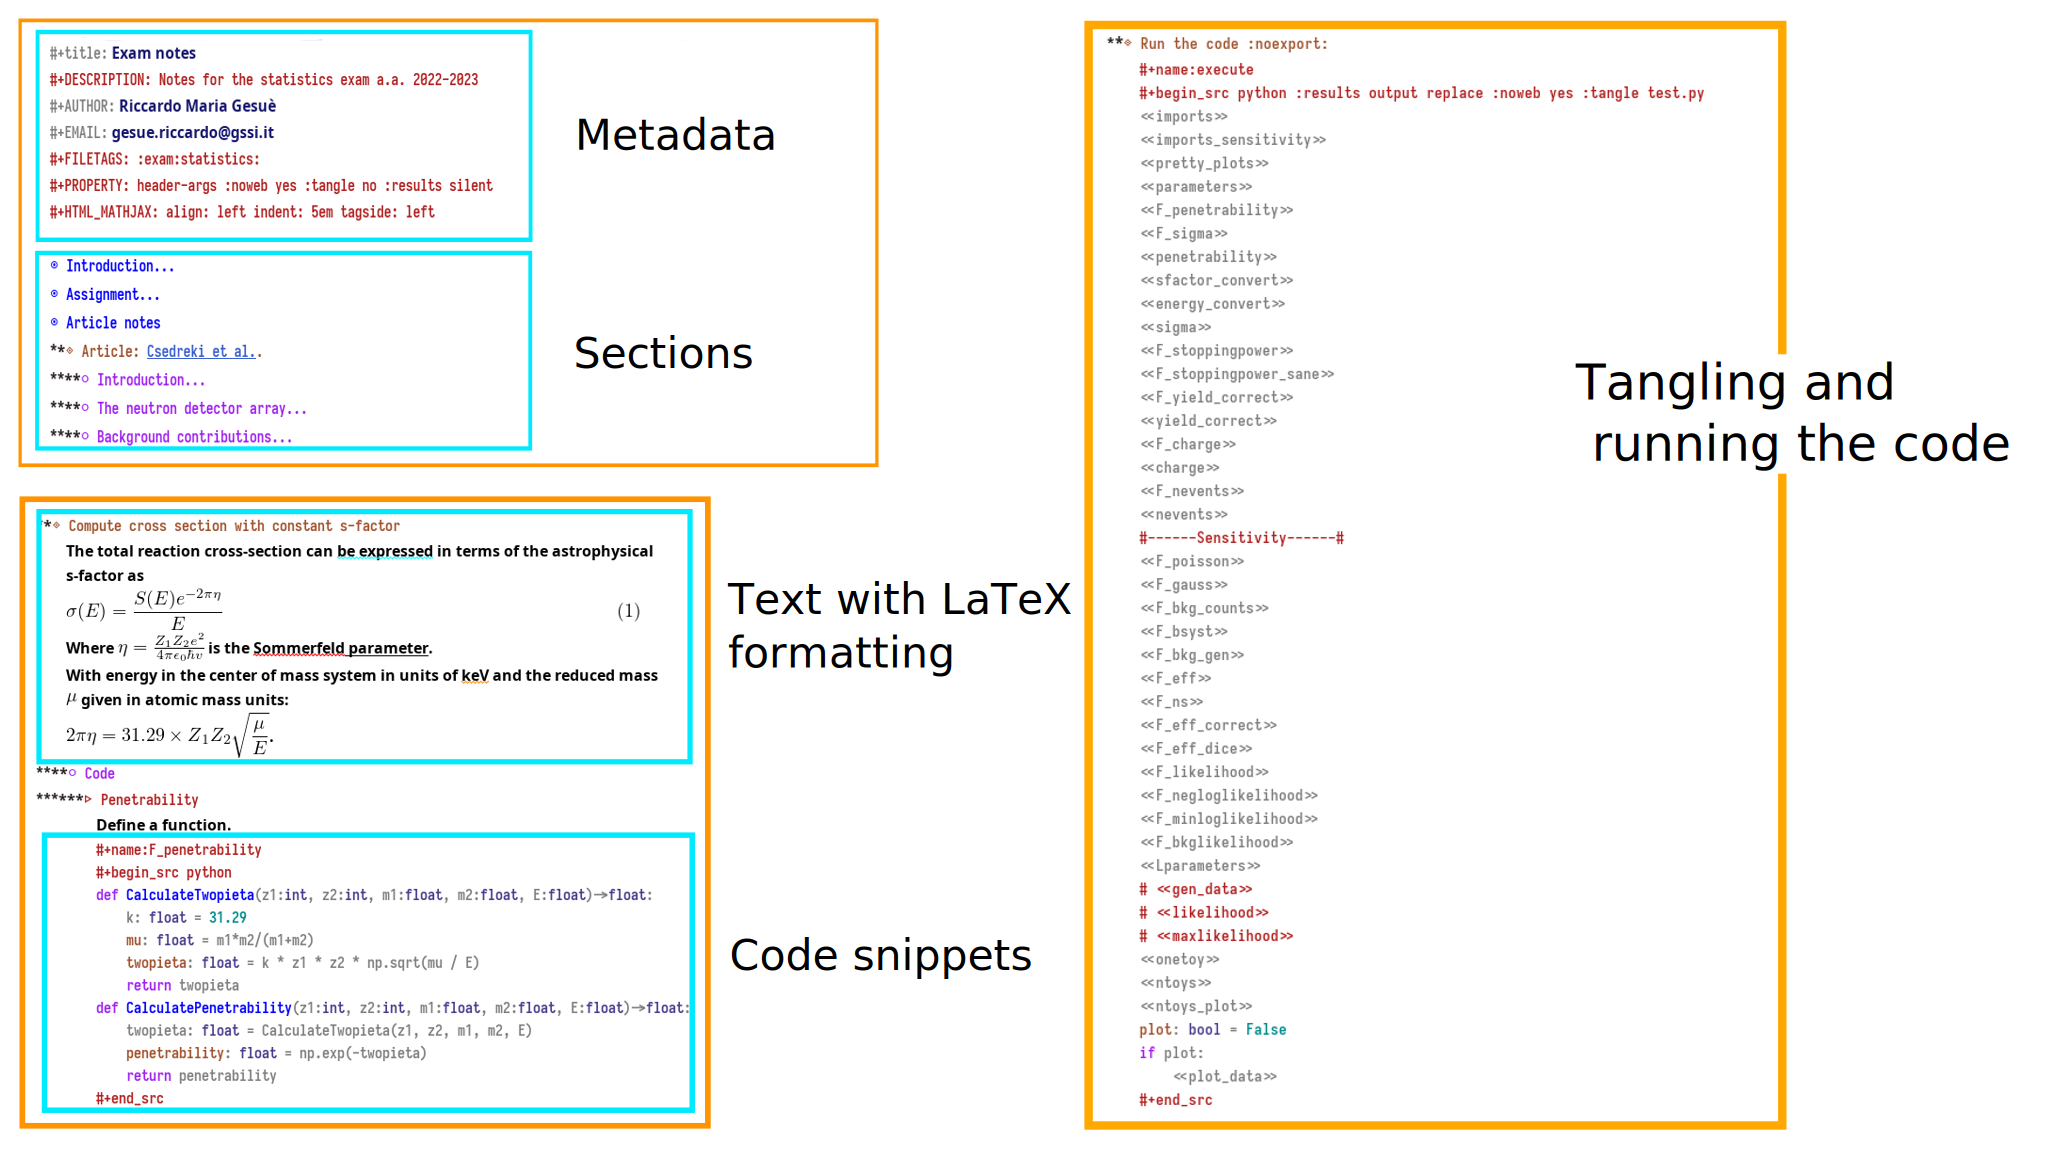
\includegraphics[width = .8\linewidth]{Images/example.pdf}
\end{frame}
\begin{frame}
  \frametitle{A first example}
  \begin{block}{}
    Typically end up with documentation file(s)
    in some \alert{readable format}
    and source file(s)
    in your \alert{language(s) of choice}.
  \end{block}
  \centering
  \includegraphics[width = .75\linewidth]{Images/html_example.pdf}
\end{frame}
%%%%%%%%%%%
\section{Why literate programming}
\begin{frame}{Advantages of literate programming}
  \begin{itemize}
    \item Focus on \alert{description} of the
          approach in human-readable form.
    \item Follow \alert{human logic} instead of
          computer logic.
    \item \alert{Understandable} code.
    \item \alert{Open and reproducible
          research}\cite{reproducibleresearch}.
    \item Very easy to go back and \alert{revise}
          an old (>2h) program.
  \end{itemize}
\end{frame}
\begin{frame}{Disadvantages of literate programming}
  \begin{itemize}
    \item Can make coding slower.
    \item Can be difficult.
    \item Can be complicated to write bigger
          programs (arguable).
    \item Not many tools.
  \end{itemize}
\end{frame}
\begin{frame}{My use case}
  \begin{itemize}
    \item Analysis in multiple steps.
    \item Not extremely complicated
          computationally.
    \item Physics/maths behind it requires
          attention.
    \item Started coding as undergrad, became more
          skilled/knowledgeable (did I?)
          during time.
    \item Show results in the most comprehensive
          and comprehensible way.
    \item \alert{Poor memory}.
  \end{itemize}
\end{frame}
%%%%%%%%%%%
\section{How to literate programming}
\begin{frame}{Tools}
  \begin{block}{}
    A literate programming tool must be able to
    execute code blocks and/or export (tangle)
    them to an executable file.
    It should make it easy to write both code
    and plain text: it must work as both
    an IDE and a writing tool.
  \end{block}
  \begin{description}
    \item[Jupyter \cite{jupyter}] It is the most
          widespread tool.
          \begin{itemize}
            \item Browser based.
            \item Developed for Python.
            \item needs extensions to work with
                  other languages(as far as I
                  know only supports C++, ROOT, R).
          \end{itemize}
    \item[Babel \cite{babel}] Functionality
          of Emacs\cite{emacs}
          org mode\cite{orgmode}.
          \begin{itemize}
            \item This is what I personally use.
          \end{itemize}
    \item[Others] Check here for a complete list:
          \url{https://literateprogramming.org}
  \end{description}
\end{frame}
\begin{frame}{GNU Emacs}
  GNU Emacs is an extensible,
  customizable text editor.
  \begin{itemize}\small
    \item You can learn more about Emacs
          functionalities here:
          \url{https://www.gnu.org/software/emacs/tour/index.html}
    \item It has notoriously a
          \alert{steep learning curve}:
          \begin{itemize}
            \item Keyboard oriented.
            \item Many different functionalities.
            \item Loads of extensions.
          \end{itemize}
    \item \textbf{But} it is
          \alert{less difficult} than
          you would think:
          \begin{itemize}
            \item Several different
                  ``distributions'' with beginner
                  friendly defaults, i.e.
                  DOOM Emacs\cite{doomemacs},
                  Spacemacs\cite{spacemacs}.
            \item Great documentation.
            \item Command prompt and intuitive
                  command names.
            \item \textit{Mouse} support.
          \end{itemize}
  \end{itemize}
  \vspace{-0.5em}
\begin{exampleblock}{}\small
Emacs is the IDE part of our tool.
\end{exampleblock}
\end{frame}
\begin{frame}{Org mode}
  \begin{block}{From the website}
A GNU Emacs major mode for keeping notes, authoring documents, computational notebooks, literate programming, maintaining to-do lists, planning projects, and more — in a fast and effective plain text system.
\vspace{1 em}

  Org is a highly flexible structured plain text file format, composed of a few simple, yet versatile, structures — constructed to be both simple enough for the novice and powerful enough for the expert.
\end{block}
\begin{exampleblock}{}
  Org is the ``plain text''/text editor
  part of our tool.
\end{exampleblock}
\end{frame}
\begin{frame}{Babel}
  \begin{itemize}
    \item Babel is Org's ability to
          \alert{execute
          and tangle} source code within
          Org documents.

    \item It was developed as a tool for
          \alert{literate programming}
          and \alert{reproducible
          research}\cite{babelarticle}.
    \item Babel supports a growing number of
          programming languages; more than
          \alert{ten dozen}
          languages currently have some Babel
          support.
    \item The core Babel functions (viewing,
          export, tangling, etc.) are
          \alert{language agnostic}
          and will work even for languages
          that are not explicitly supported.
    \item Explicit language-specific support is
          required only for \alert{evaluation}
          of code blocks in a language.
    \item Babel is designed to be
          \alert{easily extended}
          to support new languages.
  \end{itemize}
\begin{exampleblock}{}
Babel is the ``code'' part of our tool.
\end{exampleblock}
\end{frame}
\begin{frame}{Typical document structure}
  \centering
  \includegraphics[width = .9\linewidth]{Images/typical_code.pdf}
\end{frame}
%%%%%%%%%%%
\section{Useful links}
\begin{frame}[allowframebreaks]
  \frametitle{Useful links}
  \printbibliography
\end{frame}
%%%%%%%%%%%
\section{Questions}
\begin{frame}{Questions}
\end{frame}
\end{document}
